%************************************************
\chapter{All Things Classical}\label{chap:compilers}
%************************************************

Okay, maybe not \emph{all} things classical, but some things\dots
Okay, maybe just one or two really.

In this chapter we will give a very brief overview of the components of classical computers that will be helpful to further discussions of quantum circuit compilation.
A key component to quantum circuit compilation is the word ``compilation'' and its origins (in computing) span back to the early 1950's when electronic digital computers were in their early stages.
Understanding the historical development of compilation and its techniques will provide ideas and tools necessary in solving the new task of quantum circuit compilation.

This chapter is meant to provide the reader with the basics of some computing terminology and ideas.
It is by no means a complete introduction to compilers, nor computer architecture.

\section{What can a computer do?}

If you're reading this, I'm sure you can imagine something your computer is capable of.
Maybe reading this document online, sending messages/email, browsing the internet, writing documents, etc.
These are very high level operations our computer can perform, but under the hood much more primitive operations are taking place.
It is these primitive operations that we wish to understand, and will have many similarities with modern-day quantum hardware.

A simplified model of computer architecture, known as the von Neumann Architecture (\cref{fig:comparch}) shows what we now call a \ac{CPU} which is the workhorse of the computer.\footnote{At least in this \emph{very simplified} model.}

\begin{figure}[h]
    \centering
    \includestandalone[width=0.8\textwidth]{tikz/arch}
    \caption{von Neumann Architecture scheme}\label{fig:comparch}
\end{figure}

Since the \ac{CPU} is the computational piece of a computer, what can it do?
Most modern \acp{CPU} are built on the \acp{ISA} which means that the \ac{CPU} has a finite set of operations or instructions that it can perform and everything we might wish to perform on a computer, must be built up from these primitive operations.
Some examples of what these primitive operations might be are
\begin{itemize}
    \item put a value into memory,
    \item add two values in memory together and store in a new location,
    \item perform the bitwise negation on a value,
    \item compute the square root of a value.
\end{itemize}
With a set of performable operations laid out, one can then use these primitives to build up more and more complex functionality that eventually implements the things we know and love (and hate) computers for.
One thing worth mentioning here that is often glossed over in treatments of \acp{ISA} is that the instruction set must be computationally universal.\footnote{Or Turing-complete if you're computer science oriented.}
Without going too much into the weeds, we should think of computationally universal (in the classical sense) as wielding the full power of a computer, rather than only being able to do a particular type of computation.\todo{I don't like this explanation.}
Thankfully, this is relatively easy to do in the classical setting and there are even theoretical machines that use a \emph{single} operation to achieve universal computation.
\Eg{} one can achieve universal classical computation with the following instruction which implements ``subtract and branch if negative''.
\begin{lstlisting}
    Instruction subneg a, b, c
    Memory[b] = Memory[b] - Memory[a]
    if (Memory[b] < 0)
        goto c
\end{lstlisting}

While this style of architecture is great, and has worked very well, it requires the programmer to code at a very low level since the operations a \ac{CPU} performs are themselves primitive.
In order to work at a higher level of abstraction, computer scientists and programmers began to create new languages which were easier to read and write, yet could be translated into a form the brains of the computer could understand.
This would improve productivity by allowing those writing code to work at a higher level of abstraction, and bury implementation details into the code which performed the translation into the machine's instruction set.
The software responsible for translating these higher level ideas into a machines instruction set are known as \textbf{compilers}.


% With the exception of the last item, these operations are generally considered to be simple, and the latter complex.
% This has given rise to a distinction in \ac{CPU} architecture where we see \acp{CISC} and \acp{RISC}.
% The goal of the former to implement more and more complex ``primitive'' operations, while the latter leaving more work to be performed by the compiler~\cite{dragonbook}.

\section{Compilers}

While compilers have their origins in the aforementioned translation of higher level code into lower level code, they have grown considerably to perform many more tasks.
Before we dive into all of the capabilities of a modern compilers, let's take a step back and recall what the word compile means.

Merriam-Webster defines the word \textbf{compile} to mean~\cite{compiledef}
\begin{quote}
    to compose out of materials from other documents.
\end{quote}
In this context ``other documents'' might mean the higher level code itself, as well as configuration and environment variables.
With these materials the lower level machine code is then composed.
This definition is reflected in~\citetitle{dragonbook}\footnote{Colloquially known as ``The Dragon Book'' because of the cover, and likely the most famous book on (classical) compilers. This is also where the logo of the LLVM project originates from which we will discuss in~\cref{sec:llvm}.}\graffito{
    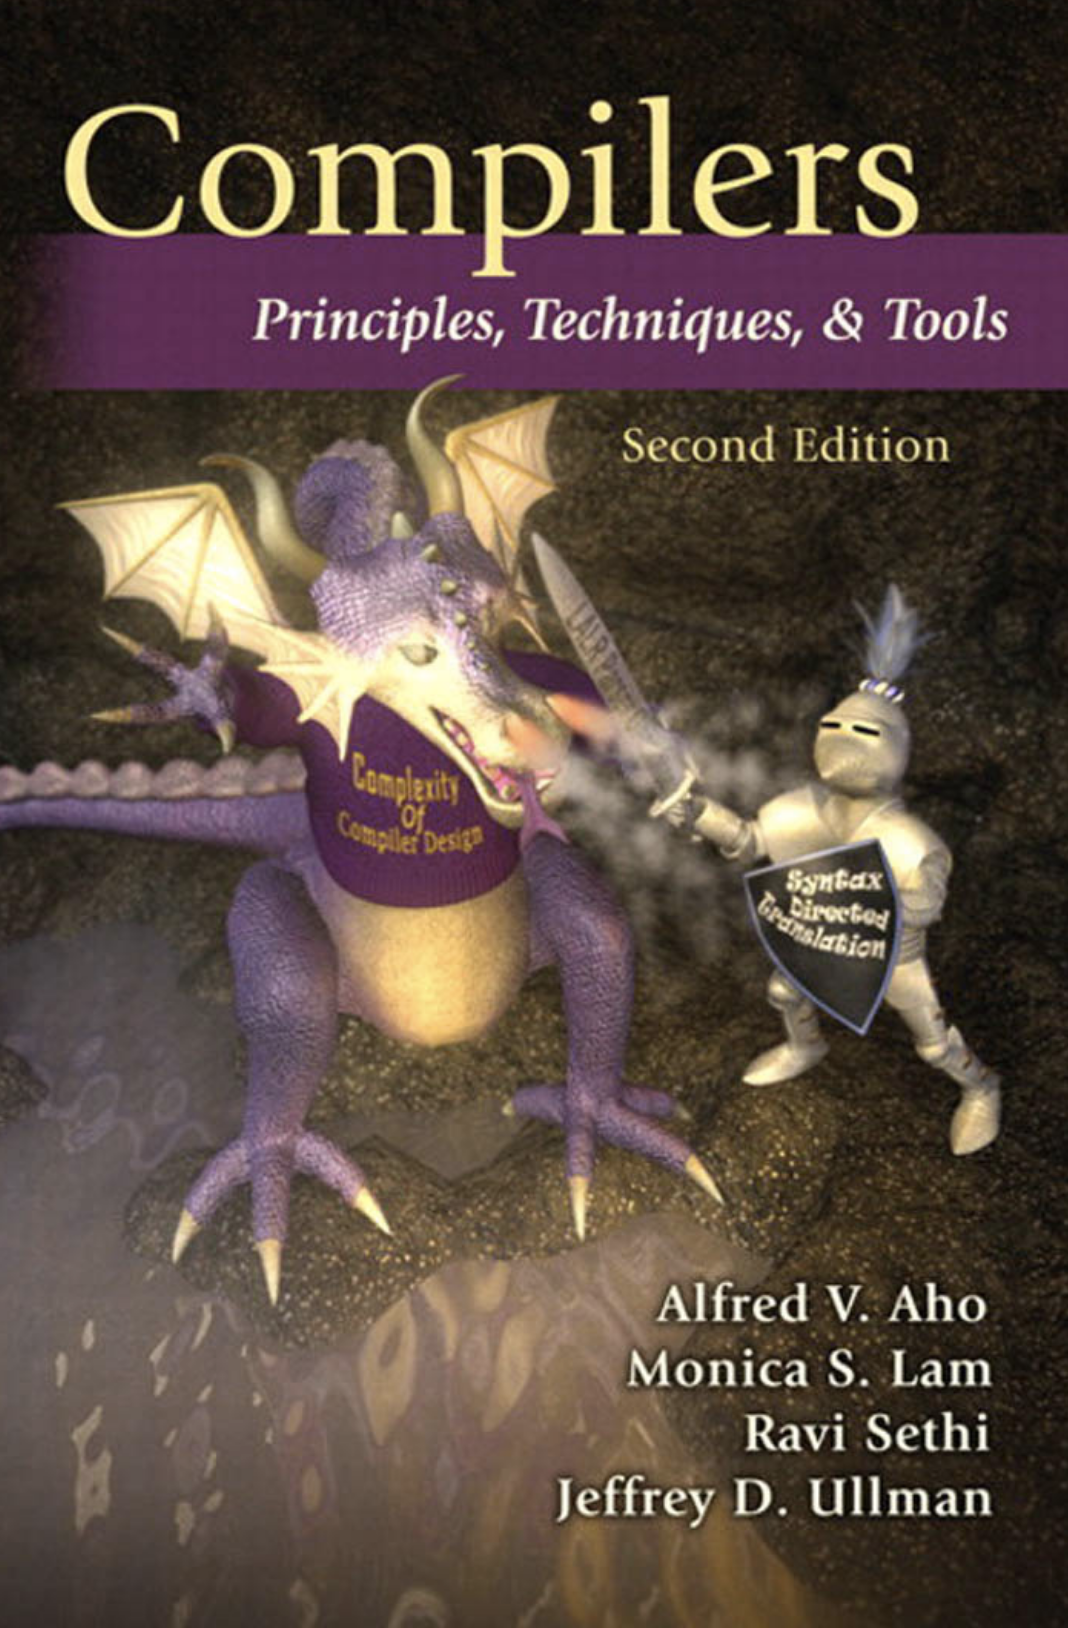
\includegraphics[width=\marginparwidth]{img/dragonbook.png}
    \emph{The Dragon Book}
    
\includegraphics[width=\marginparwidth]{img/llvmlogo.png}
    \emph{LLVM Logo}
}~\cite{dragonbook} where the authors introduce compilers through the process of transforming software.
\begin{quotation}
    [B]efore a program can be run, it first must be translated into a form in which it can be executed by a computer.

    The software systems that do this translation are called \emph{compilers}.
\end{quotation}
Hence we can view compilers as a function taking software written at one level of abstraction and bringing it down to a lower level that a computer's \ac{CPU} can understand.
\begin{figure}[ht]
    \centering
    \includestandalone[width=0.8\textwidth]{tikz/compiler}
    \caption{Action of Compiler}\label{fig:compiler}
\end{figure}

The term compiler was first used in the context computers by Grace Hopper in the early 1950's while working on a system that could translate symbolic mathematics into a machine language.
Initially Hopper's new idea was met with resistance as it was thought to be unrealistic.
\begin{quotation}
    I had a running compiler, and nobody would touch it because, they carefully told me, computers could only do arithmetic; they could not do programs.
    It was a selling job to get people to try it.
    I think with any new idea, because people are allergic to change, you have to get out and sell the idea.
    \attrib{Grace Hopper~\cite{hopperquote}}
\end{quotation}
In the end she succeeded in selling the idea and compilers have become a ubiquitous piece of modern computing infrastructure.
While Hopper's compiler focused solely on code translation, a modern compiler might perform all of line reconstruction, preprocessing, lexical analysis, syntax analysis, semantic analysis, conversion to an \ac{IR}, optimization (and there are many different types!), and finally code generation.
Thankfully we will not need to understand \emph{all} of these parts in full, but rather will focus on \aclp{IR}, optimizations, and code generation.

\subsection{Compilation Phases}

As alluded to in the previous section, a compiler has many different responsibilities.
Each responsibility is broken into a separate component so that it can be understood on it's own.
A schematic for this can be seen in~\cref{fig:compilerphases} for the main steps that we will be concerned with in this document.
\begin{wrapfigure}[24]{i}{0.25\textwidth}% TODO tweak lineheight
    \centering
    \includestandalone[width=0.23\textwidth]{tikz/phases}
    \caption{Compiler Phases}\label{fig:compilerphases} % TODO can we fix this caption?
\end{wrapfigure}

\paragraph{Syntax Analyzer}
This phase is for ensuring the code is syntactically well formed (that is it abides by the specification of the language).
If one is writing code in a binary alphabet with characters \texttt{0} and \texttt{1}, then the ``program'' \texttt{00011} is syntactically valid, while \texttt{1102} is not because a \texttt{2} appears in the code.
To complete this step many compilers turn the code into a syntax tree to complete the verification.

\paragraph{Semantic Analyzer}
Now that the code is syntactically valid we can ensure it has meaning.
This phase usually consists of type checking and scope validation (ensuring the code does not access variables outside of scope).
In some languages the operation \texttt{'hello' * 5} would pass syntax analysis, but fail semantic analysis because a string multiplied by an integer is usually not a valid operation defined.\footnote{It is completely valid in other languages like python, but python is not a compiled language.}

\paragraph{Intermediate Code Generator}
The code is now ensured to be well formed and can begin preparation to execute on hardware.
Passing directly to the code generator is sometimes possible from here, but the end product will be slower as no optimizations will take place.
From the existing code (or sometimes using the syntax tree created in the previous steps) a mid-level representation is created with the intention of being close enough to machine code that later translations are easy, and expressive enough to encompass to be optimizable.
This is best seen with a simple example.
Suppose we have the following snippet to calculate the final location of a moving object after some 5 seconds.
\begin{lstlisting}
    x_final = x_initial + velocity * 5
\end{lstlisting}
Upon transforming this code via the intermediate code generator we might end up with something like the following.
\begin{lstlisting}[label=lst:ir]
    t1 = inttofloat(5)
    t2 = velocity * t1
    t3 = x_initial + t2
    x_final = t3
\end{lstlisting}
The power here comes from the fact that the \acf{IR} can be language agnostic, and hence many languages can compile into the same \ac{IR}.
This helps us get the most out of the optimizer in the next step.

\paragraph{Code Optimizer}
Once the code is in the \ac{IR} the optimizer will attempt to improve it using many different methods.
Improve can mean many different things, but it usually refers to runtime, and memory use.
Typically optimizations that occur during this step are constant propagation, dead code elimination,
Returning to the example, upon optimization we may be left with something slightly simpler.
\begin{lstlisting}
    t1 = velocity * 5.0
    x_final = initial + t1
\end{lstlisting}
Here we have skipped the call to \texttt{inttofloat} and instead immediately converted the integer \texttt{5} to the float \texttt{5.0}.
We have also combined two of the steps to reduce the number of temporary variables we have to create and store in memory.
As you can see the task of the optimizer is not only to try and speed up the code, but reduce it's memory usage as well.
Some of the other problems the code optimizer must tackle are instruction selection, register allocation, and instruction scheduling all of which have analogs we will see in~\cref{chap:circuit-compilers}.

\paragraph{Code Generator}
Finally we have an optimized \ac{IR} and we can generate code for hardware.
This requires us to know which hardware it is we'd like to run our code on as each chip might have a different \ac{ISA}.
This is a very difficult step as many of the sub-problems that are required to be solved are themselves NP-complete such as register allocation~\cite{register-allocation-NP}. % TODO complexity
Further, generating mathematically optimal machine code has also been shown to be undecidable~\cite{dragonbook}!
Hence this step uses effective heuristics to solve the problem at hand in tractable amounts of time.
Typically this step is broken down into first optimizing the \ac{IR} for the hardware that has been chosen, followed by the actual code generation.
If this occurs the optimizer is typically referred to as hardware-independent optimizer, and a later stage of optimizations is performed in a hardware-dependent optimizer.
We will see later that the distinct phases of optimization are of crucial importance when compiling quantum circuits.

Again following the above code example, upon code generation we may end with the following generic hardware instruction code.

\begin{minipage}{0.5\textwidth}
    \begin{lstlisting}
    LDF R2, velocity
    MULF R2, R2, #5.0
    LDF R1, x_initial
    ADDF R1, R1, R2
    STF x_final, R1
\end{lstlisting}
\end{minipage}
\begin{minipage}{0.5\textwidth}
    \centering
    \begin{tabular}{cc}
        Function      & Meaning         \\ \toprule
        \texttt{LDF}  & Load float      \\
        \texttt{MULF} & Multiply floats \\
        \texttt{ADDF} & Add floats      \\
        \texttt{STF}  & Store float
    \end{tabular}
    \captionof{table}{Machine Code}\label{fig:machcode}
\end{minipage}
Here anything beginning with \texttt{R} is a register.

The phases described here are often grouped into three larger categories.
The syntax and semantic analysis, as well as the generation of an \ac{IR} fall under the umbrella of ``front end'', the optimizer is the optimizer, and everything else that follows is the ``back end''.
The implications of this design is that an optimizer and backend can be paired with many different front ends as long as the front end can generate the optimizer's preferred \ac{IR} flavor.
\begin{figure}[ht]
    \centering
    \includestandalone[width=0.75\textwidth]{tikz/frontback}
    \caption{Compiler with many front and back ends}\label{fig:compends}
\end{figure}

\subsection{Optimizations}

Before moving on to some examples of compilers, it's important to understand the separation of concerns in the two types of optimizations we've seen.
The main optimizer we see in~\cref{fig:compilerphases} as ``Code optimizer'' and again the ``Optimizer'' in~\cref{fig:compends} are typically where the majority of optimizations take place in classical compilers and are performed on an \ac{IR}.
One interesting class of examples are peephole optimizations~\cite{classical-peephole}.
These are optimizations that take advantage of small patterns found in code that can be simplified in some way.
Some examples are seen in~\cref{tab:peephole}.
\begin{table}[ht]
    \centering
    \begin{tabular}{p{.5\textwidth}l}
        Instruction                                                      & Optimized Instruction \\ \toprule
        Read value into a register, then immediately store it in memory. & Do nothing            \\
        $a \cdot x + b \cdot x$                                          & $(a + b) \cdot x$     \\
        $x - x$                                                          & $0$                   \\
        $(A^\intercal B^\intercal)^\intercal$                            & $BA$
    \end{tabular}
    \caption{Peephole Optimizations}\label{tab:peephole}
\end{table}
Other examples include dead code elimination, common subexpression elimination, and inlining.
The optimizations done here---usually to the ends of faster runtime and smaller memory use---are performed in the hopes that once the code is compiled into machine code it \emph{will} run faster.
The intuitive optimizations often remove duplication, but many other optimizations that are not so clear take advantage of the commonalities among \ac{CPU} design to produce code that will run faster on any \ac{CPU}.

With an optimized \ac{IR}, and a chosen backend, or hardware, the code can be modified to suit the instruction set, as well as other restrictions the hardware may place on computation.
\Eg{} most \acp{CPU} have a small number of registers, and hence must use them wisely throughout the computation so as to use \emph{all} of them where possible, but not slow down computation by waiting for a register to be available.
Another example is instruction scheduling where the compiler must figure out an optimal ordering to the computation, again to maximize the \acp{CPU} compute power, while not causing bottlenecks.
There are many other examples of hardware-dependent optimizations, but as you might imagine many require an intimate knowledge of the hardware's particular design.
It must do this translation all while maintaining the same semantic meaning of the original program.

In summary the first hardware-independent optimization should be thought of as optimizing the implementation theoretically, and the hardware-dependent optimization as ensuring the optimized algorithm runs as fast as possible in its final implementation.
Many more examples of optimizations (both hardware-independent and hardware-dependent) can be found in~\cite[Chapter~8]{compiler-optimizations}.

\subsection{Examples}\label{sec:compiler-examples}

We've now seen what it is a compiler is, and what we typically use it for.
A few examples are in order to help understand how compilers work in the real world, and just how varied they can be.

\begin{description}
    \item[clang:] Short for C Language, this is a compiler frontend for the C/\CPP{} languages. It takes in C/\CPP{} code and produces an LLVM \ac{IR} which we will learn about in~\cref{sec:llvm}. It then lets LLVM handle the rest of the compilation processing.
    \item[Latex:] While perhaps not very obvious, \LaTeX{} is indeed a compiler as it takes high level formatting code, and produces a lower level representation of what the user wants to typeset. Usually that comes in the form of postscript which is another programming language that is read by printers (hardware) to produce the requested document. Postscript can also be read by PDF readers and browsers which then display content as the author desired (maybe).
    \item[TensorFlow:] TensorFlow is a library for machine learning that has drawn on the design principles of compilers in attempts to speed up and ensure the accuracy of models. Indeed it has a frontend where the user builds their model and compiles it into an \ac{IR} known as HLO \ac{IR} or High Level Operations. Typical optimizations then occur and again using the LLVM compiler infrastructure this code can be brought to many backends such as the browser, mobile, and specialized compute infrastructure (such as Google's \ac{TPU}). This is all before we talk about TensorFlow Quantum which allows for hybrid quantum-classical machine learning models~\cite{tensoflowquantum}.
\end{description}

\section{LLVM}\label{sec:llvm}

The LLVM\footnote{The project, while originally an acronym for Low Level Virtual Machine now goes solely by LLVM. The original name reflects the fact that the compiler targets low level \ac{IR} code that runs on some theoretical (hence the term virtual) machine. Since the inception virtual machines have come to mean something different, hence the abandonment of the acronym.} project~\cite{llvm} is one of the largest open source compiler projects in existence and much of the compiler architecture we've discussed here come from it's design.
The founder of the project Chris Lattner has characterized compilers succinctly in~\cite{lattnerquote} as
\begin{quote}
    the art of allowing humans to think at a level of abstraction that they want to think about.
\end{quote}

Indeed as an interesting historical note, once the \ac{ISA} scheme had become commonplace, chip designers began to implement more and more complex instructions on \acp{CPU} so that machine code became higher level.
At the same time compilers became more popular, especially as their optimizations became more and more robust.
This led to a distinction between chip architectures known as \ac{CISC} and \ac{RISC}.
While \ac{CISC} \acp{CPU} are still being made and designed, they are no longer the obvious choice.
While there are many factors at play, including the economic cost of hardware vs software \ac{RISC} \acp{CPU} are becoming more popular.
Today \acp{RISC} are sometimes referred to using the backronym ``Relegate Interesting Stuff to the Compiler''.

With the growth of LLVM, developers have pushed the compiler to extend it's use to ``heterogeneous hardware''~\cite{mlir} which already includes new types of computing hardware like \acp{TPU} and could in the future encompass a \ac{QPU}.
This is exciting not \emph{just} because classical computing infrastructure is starting to think about quantum, but because this also means that our job as quantum programmers, and architects might be made easier by the monumental effort those who have come before us have built.
In quantum computing it can often feel like everything must be done from scratch as the new paradigm is so different from classical computing, yet here is a glimmer of hope we can recycle, or at the very least, learn from what has been built.
